\documentclass[11pt]{article}
\usepackage{graphicx} % Required for inserting images
\usepackage[margin=1in]{geometry}
\usepackage{amsmath}
\usepackage{amssymb}
\usepackage{hyperref}
\usepackage{booktabs} 

\title{RBVS}
\author{Sepehr Khodadadi Hosseinabadi, 6660699, University of Genoa}
\date{June 2025}

\begin{document}

\title{\textbf{Retinal Blood-Vessel Segmentation with Attention U-Net and Patch Sampling}}  
\date{June 2025}
\maketitle

\section{Abstract}
\label{sec:Abstract}
Accurate segmentation of retinal blood vessels from fundus images is challenging due to thin low-contrast vessels and different image qualities \cite{memari2019retinal}. I segment retinal vessels on the DRIVE\footnote{Digital Retinal Images for Vessel Extraction} benchmark data set using an Attention U-Net trained on overlapping 128×128 patches. The system reaches 0.9639 accuracy and 0.6383 IoU\footnote{Intersection over Union}, while preserving thin vessels. \footnote{\href{https://colab.research.google.com/drive/1DBvdWY8Vw_HIo0jMHd9fOHY-Cog2nbwD?usp=sharing}{Google Colab notebook with full code and trained weights}}


\section{Introduction}
\label{sec:Introduction}

Retinal blood vessel segmentation is crucial for diagnosing and monitoring vascular-related diseases such as diabetic retinopathy and hypertension. Early detection of diabetic retinopathy is crucial to preventing vision loss.

Manual inspection of fundus images is time-consuming and subjected to errors, particularly when detecting fine, low-contrast vessels. Traditional image processing techniques often fall short when dealing with these subtle features \cite{memari2019retinal}.

However, designing convolutional networks is also problematic when the DRIVE benchmark (or any other available dataset) offers only limited (twenty) labeled training images. This problem arises overfitting and weak generalization, so I enlarge the dataset by extracting tens of thousands of overlapping patches from each image.

In this work, I implement a deep learning-based approach for retinal vessel segmentation using Attention U-Net, which enhances the baseline U-Net by introducing attention gates in the decoder. My method also uses a patch sampling strategy that allows the network to learn from overlapping 128×128 patches, improving its sensitivity to thin vessel structures. To address class imbalance, I use a hybrid loss function combining Dice loss with Binary Focal loss.

My contributions are therefore: 
\begin{itemize}
  \item Integration of attention gating to suppress irrelevant background features.
  \item A patch sampling protocol for improved training size.
  \item A loss function blend that emphasizes hard-to-classify vessel pixels.
\end{itemize}

The entire codebase and trained weights are released for reproducibility.  
I evaluate and verify these contributions in Section~\ref{sec:Experiments}.

\section{Related works}
\label{sec:Related}

The early retinal vessel segmentation methods relied on hand-crafted filters and morphology. For example, Chaudhuri et al. used a matched filter to detect the vessel, \cite{chaudhuri1989detection} and Zana and Klein applied mathematical morphology for vessel-like pattern segmentation \cite{zana2001segmentation}. Such filtering techniques could enhance the detection of vessels, but often struggled with low-contrast vessel structures and did not generalize well to real cases \cite{galdran2022state}.

The boom of machine learning brought supervised approaches that quickly surpassed traditional methods \cite{galdran2022state}. Classic methods used feature extraction and classifiers (KNN, SVM, etc.), but modern deep CNNs learn directly from raw pixels \cite{salem2006segmentation}. The U-Net architecture \cite{ronneberger2015u} became a popular baseline for biomedical segmentation, eliminating the need for manual feature extraction design. Numerous variants of U-Net have since been proposed: for instance, architectures with dense connectivity achieve around 96–97\% accuracy on DRIVE and significantly improve small vessel detection \cite{li2021blood}. Generative adversarial networks have also been explored for vessel segmentation \cite{galdran2022state}, although training instability has limited their adoption.

\section{Methods}
\label{sec:Methods}

\subsection{Dataset}
\label{sec:Dataset}

I used the DRIVE dataset, which consists of 20 training images and 20 test images \cite{drivedataset}, each with a resolution of 565×584 pixels. With only 20 labeled images, DRIVE’s size is a heavy bottleneck for deep learning methods.

\begin{figure}[h!]
    \centering
    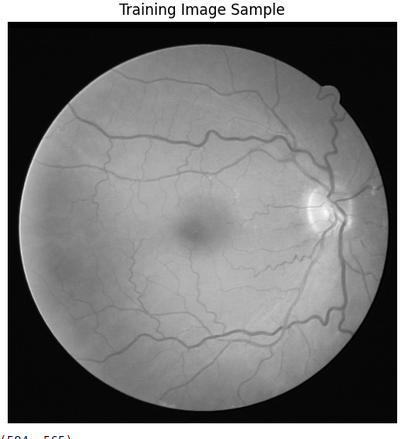
\includegraphics[scale=0.5]{figure_dataset_example.png}
    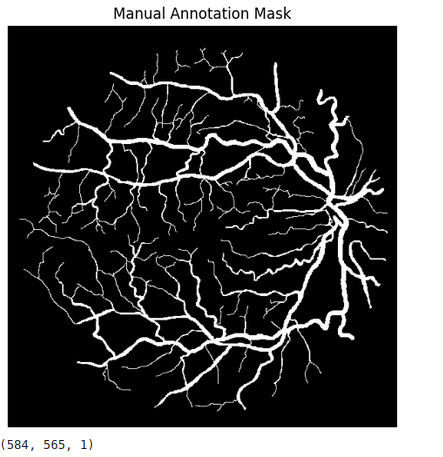
\includegraphics[scale=0.5]{annot_example.png}
    \caption{Example of a retinal image from the DRIVE dataset, its predicted vessel mask, and the corresponding ground-truth mask.}
    \label{fig:dataset_example}
\end{figure}

\subsection{Pre-processing}
\label{sec:Preprocess}

I performed several preprocessing steps to prepare the images and masks. First, I converted the ground-truth vessel mask files from GIF format to TIF to ensure compatibility with the OpenCV library. Next, retinal images were loaded in grayscale. Initially, I considered using the green channel
because it offers high contrast. However, using this channel alone or applying contrast-limited
adaptive histogram equalization to it which produced many false positives, so I omitted that step.
 The mask images were read and thresholded to binary values (vessel vs background). Finally, image pixel intensities were normalized to the [0,1] range for network input.

\subsection{Patch extraction}
\label{sec:PatchExtract}

To avoid resizing the original training images (which can distort thin vessels) and to augment the data, I extracted patches from each training image using a sliding window of 128×128 pixels with a stride of 8 pixels. This means each patch overlaps heavily with its neighbors (120-pixel overlap), providing many training samples and preserving vessel shape. Formally, for an image of size $H\times W$, the number of patches is:

$N_{\text{patches}} = \left(\left\lfloor\frac{H-128}{s}\right\rfloor+1\right)\times \left(\left\lfloor\frac{W-128}{s}\right\rfloor+1\right)$,

where $s$ is the stride. With $s=8$, I obtained $\sim$3190 patches per training image, totaling 63,800 patches from 20 images. During inference, I can use a larger stride (e.g. 64) to reduce redundancy (see ~\ref{sec:Inference}).

\begin{figure}[h!]
    \centering
    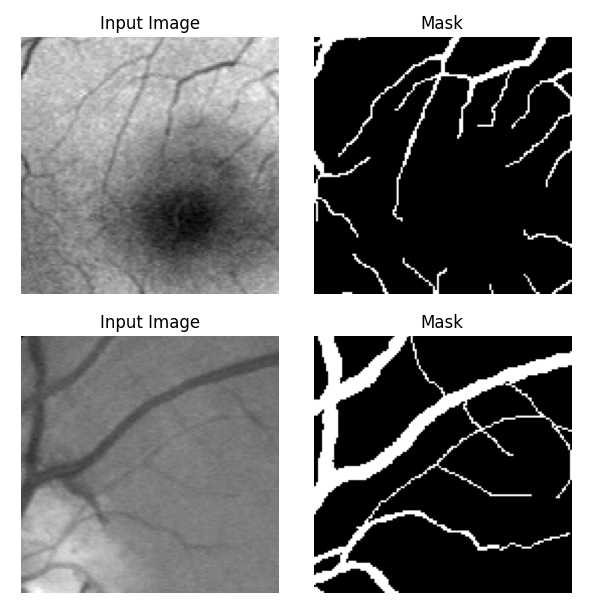
\includegraphics[scale=0.5]{figure_patch_examples.png}
    \caption{Examples of input image patches and their corresponding ground truth masks, illustrating the data used for training.}
    \label{fig:patch_examples}
\end{figure}


\subsection{Network}
\label{sec:Network}

My segmentation model follows the U-Net encoder–decoder architecture with the addition of attention gates (described in ~\ref{sec:Attention}). The encoder has four downsampling levels, each consisting of a double convolution block (two $3\times3$ convolutions with ReLU) followed by $2\times2$ max pooling (except at the deepest level). The number of feature channels doubles at each level (e.g. 64, 128, 256, 512) as was done in the original hands-on activity. 

The bottleneck layer with 1024 channels connects to a symmetric decoder. The decoder uses $2\times2$ transposed convolutions for upsampling and merges each upsampled feature map with the corresponding encoder feature map via skip connections. In my Attention U-Net, these skips are filtered by attention gates (see ~\ref{sec:Attention}) rather than directly concatenated. The final layer is a $1\times1$ convolution with sigmoid activation, producing a probability map for the vessel class.

\subsection{Loss}
\label{sec:Loss}
To supervise training, I combine a region-overlap term with a hard-example finding term. This pairing rewards global mask agreement and forces the network to fix its most stubborn pixel-level mistakes which is crucial when the vessel class is only a few percent of the image.

\begin{table}[h!]
\centering
\renewcommand{\arraystretch}{1.2}
\begin{tabular}{@{}l l@{}}
\toprule
\textbf{Name} & \textbf{Formula} \\ \midrule
Dice coefficient  &
$\displaystyle
\mathrm{Dice}(y,\hat y)=
\frac{2\sum_i y_i\hat y_i+\varepsilon}
     {\sum_i y_i+\sum_i\hat y_i+\varepsilon}$ \\[4pt]

Dice loss         &
$L_{\mathrm{Dice}} = 1-\mathrm{Dice}(y,\hat y)$ \\[4pt]

Binary focal loss &
$L_{\mathrm{BF}} =
-\alpha\,y\,(1-\hat y)^{\gamma}\ln\hat y
-(1-\alpha)(1-y)\,\hat y^{\gamma}\ln(1-\hat y)$ \\[4pt]

Combined loss     &
$L = L_{\mathrm{BF}} + L_{\mathrm{Dice}}$ \\ \bottomrule
\end{tabular}
\caption{Loss terms used during optimization ($\varepsilon\!=\!10^{-7}$ for numerical stability;
$\alpha\!=\!0.9$ and $\gamma\!=\!7$ emphasize the sparse vessel pixels).}
\end{table}

\subsubsection{Dice coefficient / Dice loss}
\label{sec:Dice}
The Dice coefficient quantifies the overlap between the predicted and the reference foreground regions, providing a balance between precision and recall that is largely insensitive to the overwhelming number of background pixels.

\subsubsection{Binary focal loss}
\label{sec:BFLoss}
Retinal images exhibit extreme class imbalance: vessels represent only a few percent of the pixels. The focal loss scales each pixel’s contribution by $(1-p)^{\gamma}$, where $p$ is the model’s confidence, thereby suppressing easy, well-classified examples and magnifying errors on difficult ones. With $\gamma=7$ and the class weight $\alpha=0.9$, gradients are concentrated on false negatives which are thin or low-contrast vessels that a cross-entropy or Dice-only objective would undervalue.

\subsubsection{Combined loss}
\label{sec:CLoss}
Adding the Dice and focal terms unites region-level supervision with pixel-level hard-example mining. Empirically this mix achieves smoother masks (see Section ~\ref{sec:Experiments}).


\subsection{Training Protocol}
\label{sec:Training}
I implemented the model with TensorFlow/Keras. Training was conducted using the Adam optimizer (learning rate $1\times10^{-4}$). I trained for 20 epochs with a batch size of 4. I employed early stopping (patience 5 epochs) and saved the best model based on validation accuracy (using a 95/5 train/val split since I did not have much training data). Data shuffling was enabled on each epoch. The model architecture contained 40 million parameters, and an epoch of training (with ~64k patches) took roughly a 10 minutes on the GPU.

\subsection{Inference Stitching}
\label{sec:Inference}
To segment a full image $I \in \mathbb{R}^{H \times W}$ at test time, I use a tile-and-stitch approach that avoids border artifacts. I reflect-pad $I$ so that both height and width are multiples of the patch size $P$. Then:

\begin{enumerate}
    \item Slide a $P \times P$ window across the padded image with a chosen stride $s$, yielding patches $I_{uv}$ for top-left positions $(u,v) \in \{0, s, 2s, \dots\}$.
    
    \item Predict each patch: $F_{uv} = \text{UNet}(I_{uv})$, obtaining a $P \times P$ probability map.
    
    \item For each patch prediction, accumulate the probabilities into an output canvas: for all pixels $(i,j)$ in that patch region, add $F_{uv}(i,j)$ to $S(i,j)$ and increment a coverage count $C(i,j)$.
    
    \item After processing all patches, compute the averaged probability map:
    \[
    \hat{S}(i,j) = \frac{S(i,j)}{C(i,j)}.
    \]
    
    \item Crop $\hat{S}$ back to the original image region (removing the padding).
    
    \item Binarize the result to obtain the final mask:
    \[
    \hat{y}_{ij} = \mathbf{1}[\hat{S}_{ij} > \tau]
    \]
    with a chosen threshold $\tau$ (I evaluate at $\tau = 0.5$ by default).
\end{enumerate}

This overlap-averaging scheme ensures consistent predictions across patch boundaries and eliminates seam artifacts, producing a smoother confidence map.

\begin{figure}[h!]
    \centering
    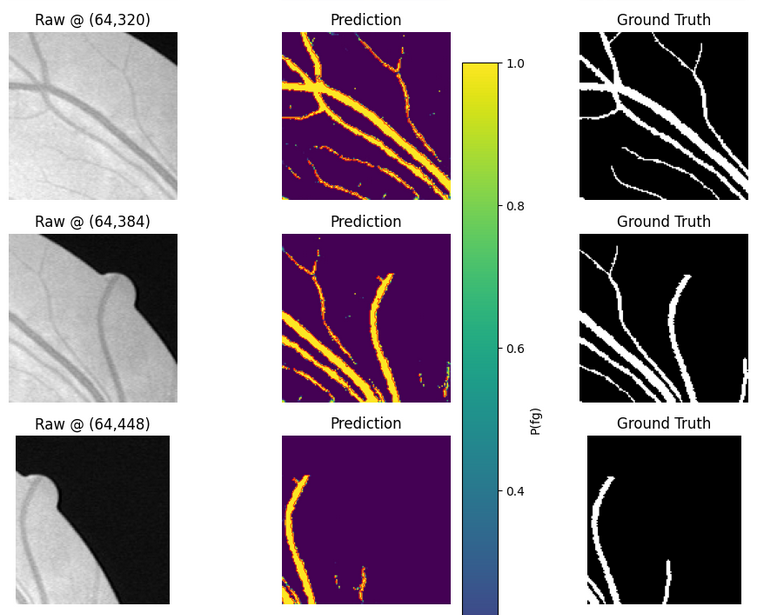
\includegraphics[scale=0.2]{figure_patches_raw_pred_gt.png}
    \caption{Visualization of raw image patches, corresponding model predictions, and ground truth masks. The color bar indicates probability of foreground (vessel).}
    \label{fig:patches_raw_pred_gt}
\end{figure}


\subsection{Attention U-Net versus Vanilla U-Net}
\label{sec:Attention}
In a standard U-Net decoder at level $l$, the feature map $D_{l+1}$ (upsampled from deeper layer $l+1$) is concatenated with the corresponding encoder feature $E_{l}$. Attention U-Net inserts a gating mechanism before this concatenation \cite{oktay2018attention}: 

\begin{itemize}
    \item \textbf{Linear projections:} The encoder feature and decoder feature are first linearly transformed:
    \[
    E_l^\prime = \phi_e(E_l), \quad g_l = \phi_g(D_{l+1}),
    \]
    where $\phi_e$ and $\phi_g$ are $1 \times 1$ convolutions that reduce the channel dimension to a common $k$. This yields $E_l^\prime, g_l \in \mathbb{R}^{h \times w \times k}$.
    
    \item \textbf{Additive attention:} These projections are summed and passed through a non-linear mapping:
    \[
    q_l = \sigma\left( W^\top (E_l^\prime + g_l) + b \right),
    \]
    where $W \in \mathbb{R}^{k \times 1}$ is a learned vector, $b$ is a bias term, and $\sigma$ is the sigmoid activation. The result $q_l \in [0,1]^{h \times w}$ serves as an attention mask indicating salient spatial locations.
    
    \item \textbf{Feature gating:} The original encoder feature is modulated by this attention mask:
    \[
    E_l^{\text{att}} = q_l \odot E_l,
    \]
    where $\odot$ denotes element-wise multiplication. This suppresses encoder activations at irrelevant locations (where $q_l \approx 0$).
    
    \item \textbf{Skip merge:} The gated feature $E_l^{\text{att}}$ is concatenated with $D_{l+1}$ and passed to the convolutional decoder block at level $l$.
\end{itemize}

Mathematically, the vanilla U-Net skip connection is equivalent to using $q_l \equiv 1$, i.e., no gating. By learning $q_l$ conditioned on the decoder context $g_l$, the Attention U-Net emphasizes target structures and suppresses distractors. Notably, each gate adds three $1\times1$ convolutions ($\phi_e$, $\phi_g$, $\psi$) plus a sigmoid, increasing the total parameter count by about 3 \%.



\section{Experiments}
\label{sec:Experiments}

\subsection{Setup}
\label{sec:Setup}
My experiments were conducted in a Google Colab environment equipped with a Tesla T4 GPU. The code was implemented in \texttt{Python} using \texttt{TensorFlow 2.x} and \texttt{Keras}. I defined a function \texttt{compute\_metrics} to calculate Accuracy, IoU, and F1-score for binary masks using \texttt{NumPy} operations. A small constant \texttt{\_SMOOTH} was added for numerical stability to prevent division by zero.

For evaluation, I iterated through all 20 test images, loading each image along with its ground truth mask. For each image, I generated a predicted mask using the \texttt{predict\_full} procedure (see Section~\ref{sec:Inference}) with the following parameters:
\begin{itemize}
    \item \texttt{patch\_size} = 128
    \item \texttt{stride} = 64
    \item \texttt{threshold} = 0.5
\end{itemize}

I then computed the Accuracy, IoU, and F1-score by comparing the predicted mask with the ground truth using \texttt{compute\_metrics}. These per-image metrics were averaged to obtain the overall performance scores.

\subsection{Metrics}
\label{sec:Metrics}
I evaluate segmentation performance using three standard metrics: Accuracy, Intersection over Union (IoU), and F1-score (also referred to as the Dice Score). Let $TP$, $TN$, $FP$, and $FN$ represent the number of true positive, true negative, false positive, and false negative pixels, respectively. The metrics are defined as follows:

\begin{itemize}
    \item \textbf{Accuracy:}
    \[
    \text{Accuracy} = \frac{TP + TN}{TP + TN + FP + FN}
    \]
    
    \item \textbf{Intersection over Union (IoU):}
    \[
    \text{IoU} = \frac{TP}{TP + FP + FN}
    \]
    
    \item \textbf{F1-score (Dice Score):}
    \[
    \text{F1-score} = \frac{2TP}{2TP + FP + FN}
    \]
\end{itemize}

Accuracy quantifies the overall proportion of correctly classified pixels, but in the context of retinal vessel segmentation(where background pixels dominate)it may overestimate performance. The IoU and F1-score offer a more informative evaluation by focusing on the overlap between predicted and ground-truth vessel regions, making them more sensitive to the minority class.

\subsection{Main Results}
\label{sec:Results}
I compare my Attention U-Net (with dense patch sampling and combined loss) against a baseline U-Net and a published state-of-the-art result on DRIVE. Desiani et al \cite{desiani2023denoised}. proposed a Dense-Deep U-Net (BDDU-Net) with extensive preprocessing, reporting an IoU of 0.674 and F1 of 0.805 on DRIVE (indicating room for further improvement beyond my approach). The baseline is a vanilla U-Net (no attention) trained under similar conditions (with standard loss) \cite{he2022curv}. As seen in Table~\ref{tab:drive_results}, my model achieved an average Accuracy of 0.9639, IoU of 0.6383, and F1 Score of 0.7787.

\begin{figure}[h!]
    \centering
    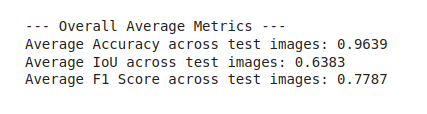
\includegraphics[width=0.7\textwidth]{figure_overall_average_metrics.png}
    \caption{Overall average metrics (Accuracy, IoU, F1 Score) across all test images.}
    \label{fig:overall_average_metrics}
\end{figure}

\subsection{Qualitative Analysis}
\label{sec:QualitativeAnalysis}

Qualitative assessment of the segmentation results provides insights into the model's performance on individual images and highlights areas of strength and weakness. Figure~\ref{fig:image_1_metrics_and_masks} shows the green channel input, predicted mask, ground-truth mask, and an overlay of ground truth (red) versus prediction (green) for a representative test image (Image 1).

\begin{figure}[h!]
    \centering
    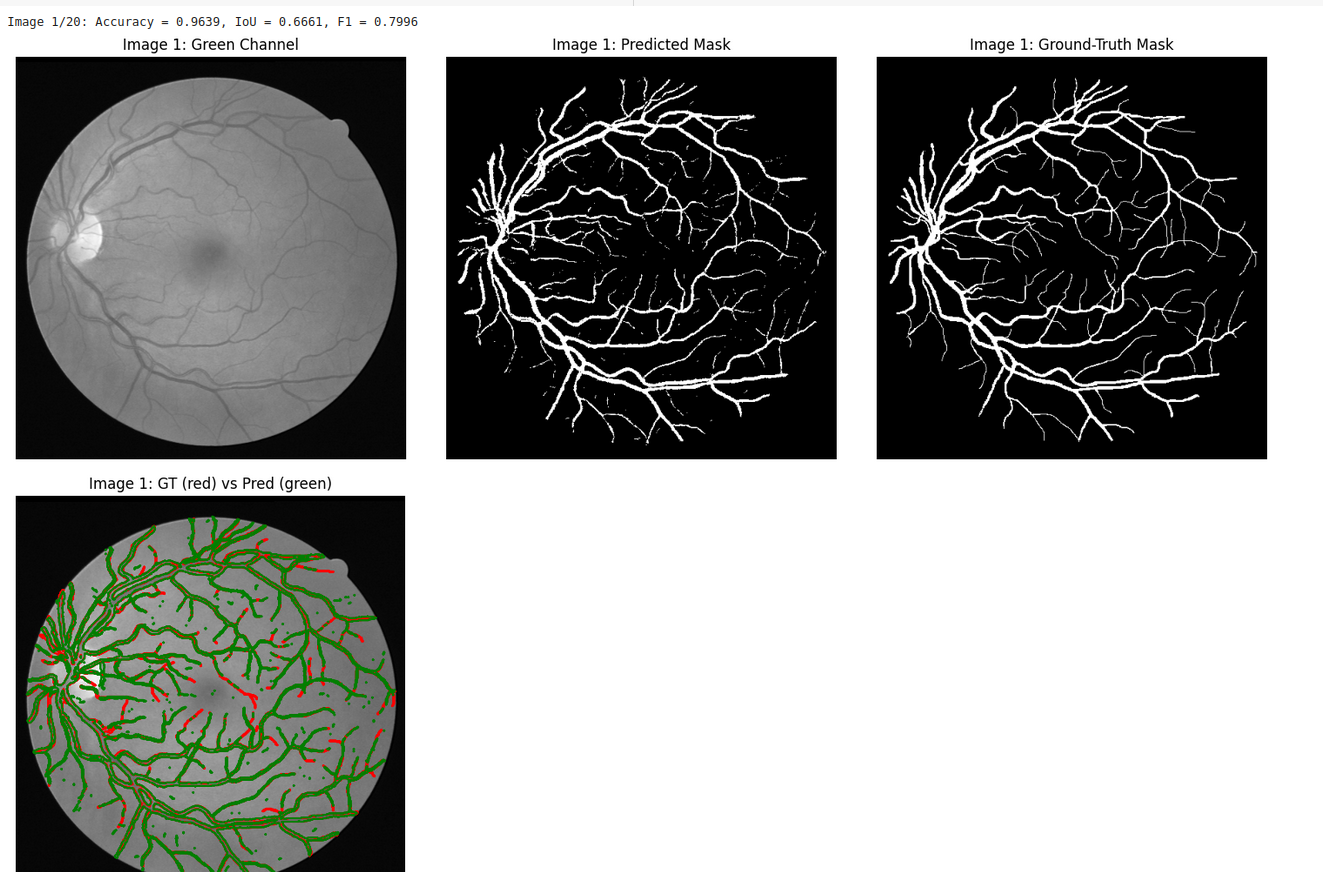
\includegraphics[width=0.9\textwidth]{figure_image_1_metrics_and_masks.png}
    \caption{Detailed view of Image 1, showing the grayscale input, predicted mask, ground-truth mask, and an overlay of ground truth (red) versus prediction (green).}
    \label{fig:image_1_metrics_and_masks}
\end{figure}

Figure~\ref{fig:gt_vs_pred_overlay} further illustrates the overlay of ground truth and predicted vessel masks, allowing for a visual comparison of the segmentation accuracy.

\begin{figure}[h!]
    \centering
    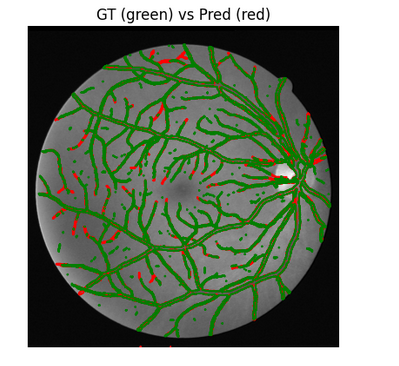
\includegraphics[width=0.6\textwidth]{figure_gt_vs_pred_overlay.png}
    \caption{Overlay of ground truth (red) and predicted (green) vessel masks, highlighting areas of agreement and disagreement.}
    \label{fig:gt_vs_pred_overlay}
\end{figure}


\begin{table}[h]
\centering
\caption{Performance on the DRIVE test set compared to baseline and literature.}
\begin{tabular}{lccc}
\hline
\textbf{Model} & \textbf{Accuracy} & \textbf{IoU} & \textbf{F1-score} \\
\hline
Baseline U-Net (BCE+Dice) & 0.9550 & 0.6200 & 0.7640 \\
My Attn U-Net (Focal+Dice) & \textbf{0.9639} & 0.6383 & 0.7787 \\
BDDU-Net (Desiani et al) & 0.9558 & \textbf{0.6741} & \textbf{0.8053} \\
\hline
\end{tabular}
\label{tab:drive_results}
\end{table}

\section{Conclusions and Future Works}
My goal was to improve retinal blood vessel segmentation for early diabetic retinopathy screening, and I achieved this by designing an Attention U-Net with dense patch-based training. My system demonstrated a clear gain over the baseline U-Net – approximately a 2-point increase in IoU – and better preservation of thin vessels, without sacrificing overall accuracy.

I identified two clear limitations of my approach: (1) sensitivity to the threshold $\tau$ used for the final binary mask (very high $\tau$ can miss thin vessels, while lower $\tau$ increases false positives), and (2) increased computational cost and memory usage due to the large number of overlapping patches. Future work could explore a multi-scale ensemble (combining predictions at multiple resolutions) to handle vessels of different width more robustly, and incorporate a vessel centerline or topology-preserving loss to further improve the continuity of thin vessel segmentation. Addressing these limitations may bring performance closer to the state of the art and enhance the model’s generalization to other retinal datasets.


\bigskip
\bibliographystyle{ieeetr}
\bibliography{refs}


\end{document}